\documentclass[a4paper,11pt]{article}  %11pt
\pdfoutput=1 % if your are submitting a pdflatex (i.e. if you have
             % images in pdf, png or jpg format)

\usepackage{jheppub2} 
%\usepackage{jheppub} % for details on the use of the package, please
                     % see the JHEP-author-manual

\usepackage[T1]{fontenc} % if needed

\usepackage[utf8]{inputenc} 

\usepackage{amsfonts}
\usepackage{booktabs}
\usepackage{siunitx}

%%%%%%%%%%%%%%%%%%%%%%%%%%%%
\usepackage{caption} %To include caption in tabular
% Packages required to draw diagrams with TikZ
%\usepackage{geometry}            
% See geometry.pdf to learn the layout options. There are lots.
\usepackage{graphicx}
\usepackage{amsmath}
\usepackage{amssymb}
\usepackage{multicol}
\usepackage{slashed}
\usepackage{tcolorbox}

\usepackage{listings}
\usepackage{color}

\definecolor{dkgreen}{rgb}{0,0.6,0}
\definecolor{gray}{rgb}{0.5,0.5,0.5}
\definecolor{mauve}{rgb}{0.58,0,0.82}

\lstset{frame=tb,
  language=Python,
  aboveskip=3mm,
  belowskip=3mm,
  showstringspaces=false,
  columns=flexible,
  basicstyle={\scriptsize\ttfamily},
  numbers=none,
  numberstyle=\tiny\color{gray},
  keywordstyle=\color{blue},
  commentstyle=\color{dkgreen},
  stringstyle=\color{mauve},
  breaklines=true,
  breakatwhitespace=true,
  tabsize=3
}


\newtcolorbox{redbox}[1]{colback=red!5!white,colframe=red!75!black,fonttitle=\bfseries,title=#1}

\newtcolorbox{bluebox}[1]{colback=blue!5!white,colframe=blue!75!black,fonttitle=\bfseries,title=#1}

\newtcolorbox{yellowbox}[1]{colback=yellow!5!white,colframe=yellow!75!black,fonttitle=\bfseries,title=#1}


\def\sst{\scriptscriptstyle}

\newcommand{\comm}[1]{{\color{red}\bf[#1]}}
\newcommand{\answer}[1]{{\color{blue}\bf[#1]}}

\newcommand{\beq}{\begin{equation}}
\newcommand{\eeq}{\end{equation}}
\newcommand{\eV}{\,{\rm eV}}

\newcommand{\SU}{\,{\rm SU}}
\newcommand{\SO}{\,{\rm SO}}
\newcommand{\Sp}{\,{\rm Sp}}
\newcommand{\U}{\,{\rm U}}
\newcommand{\N}{N_c}


%%%%%%%%%%%%%%%%%%%%%%%%%%%%
% BIBLIOGRAPHY STYLE
\usepackage{natbib}
 \bibliographystyle{JHEP} %for [1], [2] etc.
%\bibliographystyle{apalike}
%%%%%%%%%%%%%%%%%%%%%%%%%%%%


\preprint{}

\title{\boldmath Algorithmic Trading}

% more complex case: 4 authors, 3 institutions, 2 footnotes
\author{Alexis D. Plascencia}

% The "\note" macro will give a warning: "Ignoring empty anchor..."
% you can safely ignore it.

%\affiliation[]{Physics Department and Center for Education and Research in Cosmology and Astrophysics (CERCA), 
%Case Western Reserve University, Cleveland, OH 44106, USA}

% e-mail addresses: one for each author, in the same order as the authors
\emailAdd{aplascenciac@gmail.com}

\abstract{Overview of algo trading.}

\begin{document} 
\maketitle
\flushbottom
\clearpage

\section{Moving average crossover}

\textbf{Trend following} buys when an asset’s price rises and goes short when an asset’s price falls. Trend following strategies often result in numerous small losses, with infrequent but substantial gains that compensate for these losses. \\

Moving average crossover is a trend following strategy. Crossovers use two different moving averages, for example, 100 days and 25 days. When the smaller moving average crosses above the larger moving average (when the 25-day crosses over the 100-day), a buy signal occurs. When the shorter moving average crosses below the larger moving average, this can be used as a sell signal.\\

Dual Moving Average strategy: As the name implies, the system uses two moving averages: a 100-day moving average and a 350-day moving average. This system is always in the market: Long when the shorter moving average is above the long moving average and vice versa. (We have backtested moving average trading strategies.) \\

\section{Momentum}

This is a trend following strategy. The aim is to long signal when the price reaches the highest price for the last \texttt{window\_size} days. Short signal when the price reaches its lowest point. We get out of the position when the prices crosses the moving average of the last \texttt{window\_size} days. \\

\begin{redbox}{Data preprocessing}
\begin{lstlisting}
def process_data(data, window_size=36):
    # Assuming 'data' is a DataFrame
    data["high"] = data["close"].shift(1).rolling(window=window_size, center=False).max()
    data["low"] = data["close"].shift(1).rolling(window=window_size, center=False).min()
    data["avg"] = data["close"].shift(1).rolling(window=window_size, center=False).mean()

    data["long_entry"] = data["close"] > data["high"]
    data["short_entry"] = data["close"] < data["low"]

    data["long_exit"] = data["close"] < data["avg"]
    data["short_exit"] = data["close"] > data["avg"]
    return data

\end{lstlisting}
\end{redbox}


\begin{bluebox}{Momentum strategy}
\begin{lstlisting}
def strat(data):
  ''' **Momentum strategy**: Long signal when the price reaches the highest price for the last window_size days.Short signal when the price reaches its lowest point.We get out of the position when the prices crosses the moving average of the last window_size days.'''
  
  l_signals = []
  position = 0
  for k in range(len(data["close"])):
    if data["long_entry"][k] and position==0:
      l_signals.append(1)
      position = 1
    elif data['short_entry'][k] and position==0:
      l_signals.append(-1)
      position = -1
    elif data["long_exit"][k] and position>0:
      l_signals.append(-1)
      position = 0
    elif data["short_exit"][k] and position<0:
      l_signals.append(1)        
      position = 0
    else:
       l_signals.append(0)
\end{lstlisting}
\end{bluebox}

\begin{tabular}{lSS} \toprule
\textbf{ Momentum Strategy}  &  \text{2020-2023} & \text{2018-2022}\\ \midrule
Initial Balance & 1000 & 1000\\
Profit (\%) & 493.33 &  2029.45\\  
Trades Executed &  14 & 15\\
Maximum Drawdown (\%) &  21.01 & 5.35\\
Average Drawdown (\%) &  4.09&0.55 \\

Maximum PNL &  1743.41&   6065.84\\
Minimum PNL &  -1488.36&  -111.78\\
Max Portfolio Balance  & 7510.99 & 21294.53\\
Minimum Portfolio Balance &  1000.00& 985.7\\ 
Total Fee &  77.51 & 150.56\\ \midrule
Final Balance &   \textbf{5933.28}& \textbf{21294.53} \\ \bottomrule
\end{tabular}

\section{Mean reversion}

Mean reversion is a market neutral strategy, or neutral trend. The underlying idea is that prices revert toward the mean.
Extreme events are followed by more normal events. We will find a time where a value
such as the price or the return is very different from the past values. Once established, we
will place an order by forecasting that this value will come back to the mean.\\

Mean reversion strategy: This strategy assumes that the value of a price/return
will return to the average value. \\

Unlike the mean reversion strategy, \textbf{pair trading}-mean reversion is based on the
correlation between two instruments. If a pair of stocks already has a high
correlation and, at some point, the correlation is diminished, it will come back to
the original level (correlation mean value). If the stock with the lower price
drops, we can long this stock and short the other stock of this pair.\\



In order to trade using this strategy, we need to quantify what it means for the price to be higher or lower than expected. It's useful to compute the z-score of the price on each day, which tells us how many standard deviations away from the mean a value is:
$$ z = \frac{x - \mu}{\sigma} $$

where $x$ is the value, $\mu$ is the mean of the data set, and $\sigma$ is its standard deviation. So a price with a $z\text{-score }> 1$ is more than one standard deviation above the mean, and we will sell short when this happens. If the price on a day has a $z\text{-score }< 1$, we will buy long. If the price is within half a standard deviation of the mean, we will clear all positions

\begin{align}
z\text{-score }> 1 & \implies {\rm short} \nonumber\\
z\text{-score }< 1 &\implies {\rm long} \nonumber\\
|z\text{-score}| < 0.5 &\implies \text{close position} \nonumber
\end{align}


The danger of applying mean reversion to a single asset is that it exposes us to the movement of the market and the success or failure of the individual asset, among other factors. If there is a persistent trend affecting the price of the security, we will find ourselves consistently undervaluing (if the price is moving steadily upward) or overvaluing (if the price is falling) the asset. One strategy to mitigate this risk is to consider a basket of different assets.\\


\section{Bollinger Bands}

When the price of the asset breaks below the lower band of the Bollinger Bands, prices have perhaps fallen too much and are due to bounce. On the other hand, when price breaks above the upper band, the market is perhaps overbought and due for a pullback.\\

Using the bands as overbought/oversold indicators relies on the concept of mean reversion of the price. Mean reversion assumes that, if the price deviates substantially from the mean or average, it eventually reverts back to the mean price.\\

Price often can and does "walk the band". In those markets, traders who continuously try to "sell the top" or "buy the bottom" are faced with an excruciating series of stop-outs, or even worse, ever-mounting losses as price moves further and further away from the original entry.\\

This is an example of a Bollinger Band for bitcoin prices:
$$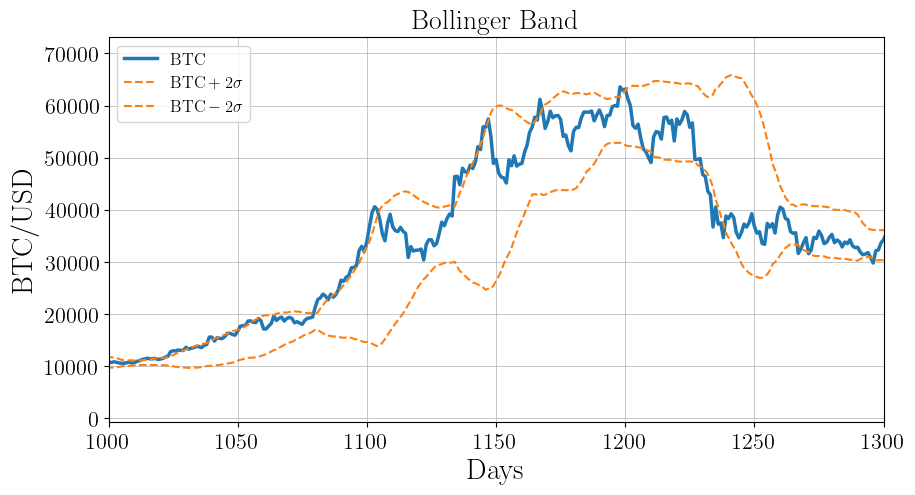
\includegraphics[width=0.85\textwidth]{bollinger.png} $$

\section{Triple Moving Average strategy}

This system uses three moving averages: 150, 250, and 350-day moving averages. Buy and sell occur when the 150-day moving average breaks above and below the 250-day moving average. The 350-day average is used as a trend filter: Trades happen only when both moving averages are on the same side as the longer 350-day average. If both are higher, long trades are permitted. If both are lower, only short trades are permitted.


\section{Volatility Modulation}

One of the primary measures of a PM's risk capacity is the trading stop: the number of chips the PM has to play with. Why, then should a PM who runs 4\% volatility when 5\% away from the stop take the same level of risk when 10\% away from the stop? It is natural to assume the level of risk (volatility $\sigma$) should be proportional to the distance from the stop, and that as this distance increases, so should the risk taken by the PM. This is a strategy called \textbf{volatility modulation}.\\ 

\noindent The level of risk depends only on the year-to-date return on notional:
$$ r(t) = \frac{{\rm P\&L}}{N} $$ 
and the linear modulation for the volatility is given by
$$ \sigma = \sigma_0 + m \frac{\sigma_0 r(t)}{D_0}$$
when $m>1$ there is strong modulation which works for PM who are adverse to risk, there is increased risk tolerance on the upside and small risk tolerance on the downside. However, if $m\gg 1$ is counterproductive since it makes the PM extremely risk adverse when there are losses.\\

The optimal linear modulation strength only depends on the PM's risk tolerance. For our choice of objective, it can be shown analytically that the optimal strength is independent of the Sharpe ratio as long as 
$$ \frac{\sigma_0}{D_0} \leq \sqrt{2 \left[ \log(1+k)- \frac{k}{1+k} \right] } $$
where the hurdle is $k\times$ the trading stop.
$$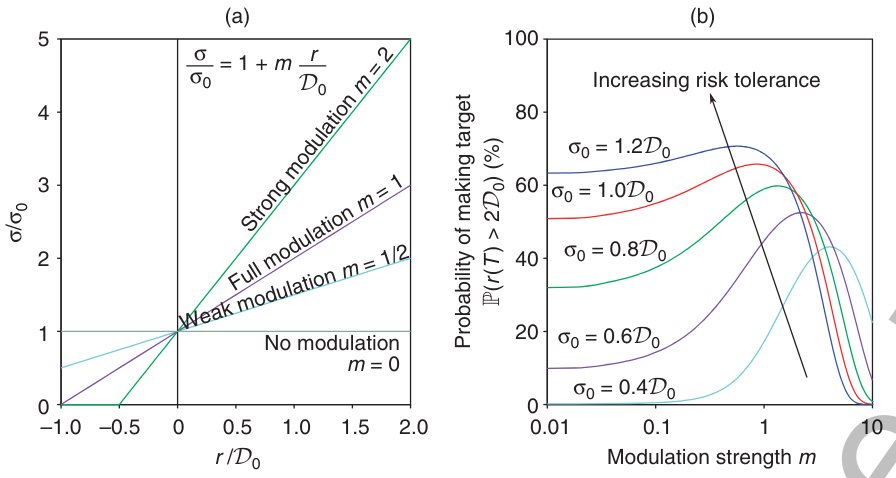
\includegraphics[width=0.85\textwidth]{vol-modulation.png} $$

%%%%%%%%%%%%%%%%%%%%%%%%%%%%%%%%%%%%%%%%%%%%%%%%%%%%%%%%%%%%%%%%%%%%%%%%%%%%%%%%
%%%%%%%%%%%%%%%%%%%%%%%%%%
% BIBLIOGRAPHY
% REMEMBER TO WRITE THE LINE bibtex article IN THE TERMINAL TO GENERATE THE 
% CORRESPONDING FILES
\bibliography{Random}
%%%%%%%%%%%%%%%%%%%%%%%%%%%%

%\begin{thebibliography}{99}
% Please avoid comments such as "For a review'', "For some examples",
% "and references therein" or move them in the text. In general,
% please leave only references in the bibliography and move all
% accessory text in footnotes.
% Also, please have only one work for each \bibitem.
%\end{thebibliography}

\end{document}

